\documentclass{beamer}

\definecolor{Burgandy}{RGB}{134,0,56}
\mode<presentation>
{
\usetheme{Madrid}
\setbeamercolor*{palette primary}{use=structure,fg=white,bg=Burgandy}
\setbeamercolor*{palette secondary}{use=structure,fg=white,bg=Burgandy}
\setbeamercolor*{palette tertiary}{use=structure,fg=white,bg=Burgandy}
}

\usefonttheme{professionalfonts} % using non standard fonts for beamer
\usefonttheme{serif} % default family is serif
\usepackage{amssymb}
\usepackage{hyperref}
\usepackage{amsfonts}
\usepackage{graphicx}
\usepackage{multimedia}
%\usepackage{subfig}
\usepackage{mathrsfs}
\usepackage{enumerate}
\usepackage{tikz}
%\usepackage{epstopdf}
\usepackage{mathtools}
%\usetikzlibrary{matrix}

\newcommand{\id}{\mathrm{id}}
\newcommand{\dd}{\mathrm{d}}
\date{}
\mode<presentation> {
\setbeamertemplate{navigation symbols}{}
}
\begin{document}
\section{Spring Pendulum}
\begin{frame}[noframenumbering]{ \hspace{1pt}}

\begin{center}
\huge Characterizing a Spring Pendulum \\ with Monte Carlo Methods \\
\vspace{12 pt}
\normalsize Dawn Sargent (Fairmont State University)

{\small MAA Allegheny Mountain Section Conference, Penn State Behrend

6 April 2018}
\end{center}
\end{frame}

\begin{frame}{Special Thanks}
\centering
\begin{minipage}{0.3\textwidth}
	
\includegraphics[scale=0.3]{images/FSULogo.jpg}
\end{minipage} \quad
\begin{minipage}{0.3\textwidth}
	
\includegraphics[scale=0.25]{images/NasaLogo.jpeg}
\end{minipage} \quad
\begin{minipage}{0.3\textwidth}
	
\includegraphics[scale=0.1]{images/NVidiaLogo.jpg}
\end{minipage}
\end{frame}

\begin{frame}{The Problem}
\center
What makes a spring pendulum result in chaotic motion? \newline

$\ \ \ \ \ \ x'' + \frac{k}{m}x - (l+x)\theta'^2 - g \cos\theta = 0$ \\ 
\vspace{12 pt}
$\ \ \ \ \ \ \theta'' + \frac{g \sin\theta + 2x'\theta'}{l+x} = 0$ \\
\vspace{15 pt}
    \begin{tabular}{| c | c | c | c |}
    \hline
    Variable & Description & Distribution & Units \\ \hline
    $x(0)$ & initial stretch & $N(0.1, 0.01)$ & $m$ \\ 
    $\theta(0)$ & initial angle from vertical & $N(10, 0.6)$ & $deg$ \\ 
    $m$ & pendulum mass & $N(1, 0.1)$ & $kg$ \\ 
    $k$ & spring constant & $N(30, 0.25)$ & $N/m$\\ 
    $g$ & acceleration due to gravity & $N(9.8, 0.1)$ & $m/s^2$ \\ 
    $l$ & unstretched length & $N(1, 0.1)$ & $m$\\ \hline
\end{tabular}
\end{frame}

\iffalse
\begin{frame}{Monte Carlo Simulation}
\begin{center}
Monte Carlo methods can be very useful for numerically modeling physics-related problems such as this that involve so many degrees of freedom, or independently varied parameters. To perform a Monte Carlo simulation, we identify meaningful ranges for each parameter involved and the algorithm randomly chooses from each. Doing this a very large number of times, by the Law of Large Numbers, we are able to obtain results very close to the actual expected outcomes and their associated probabilities. \\ 
\vspace{15 pt}
\href{VIDEO}{VIDEO}
\end{center}
\end{frame}
\fi

\begin{frame}{Performance Metric}
\centering
In order to identify what parameters effect the success of a trial, we must first determine what will define a success versus a failure.\newline \newline
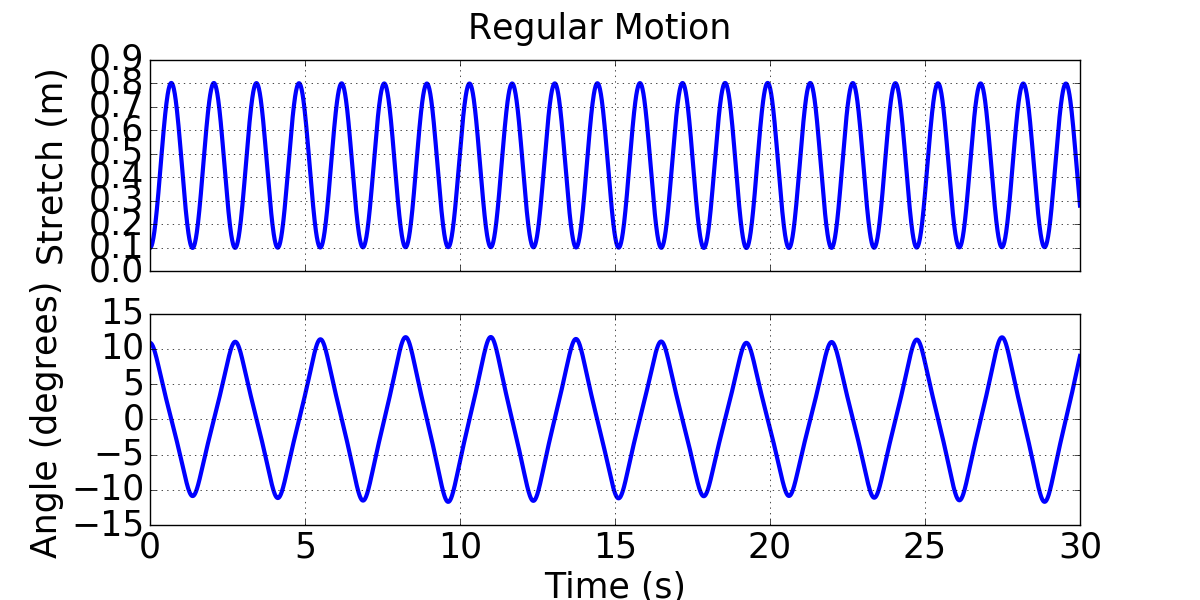
\includegraphics[scale=0.18]{images/RegularMotion.png} 
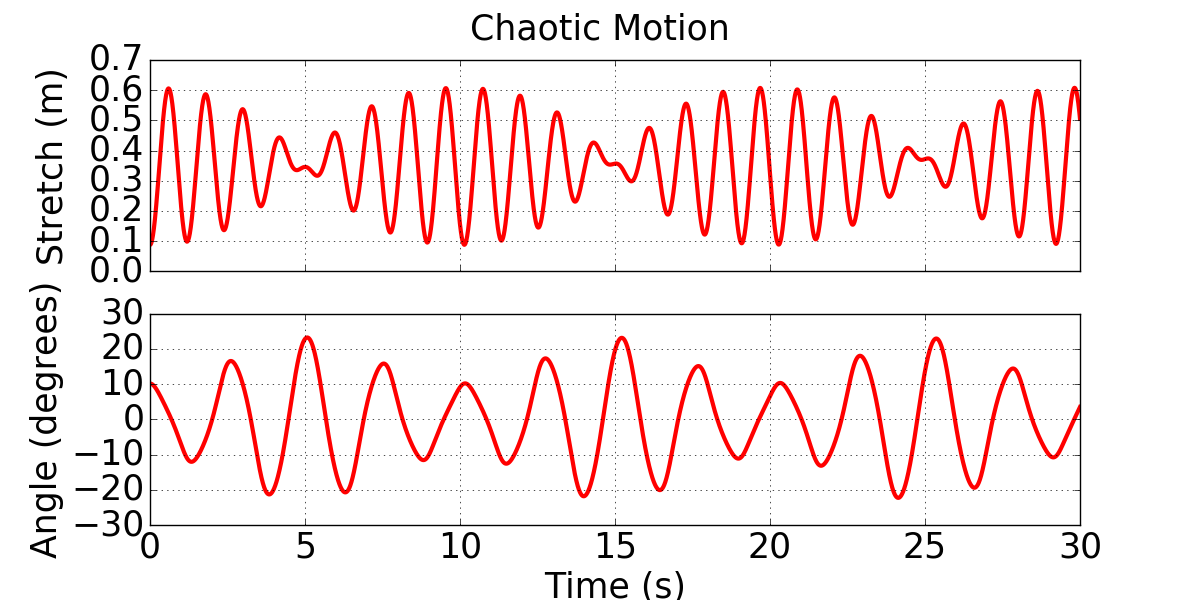
\includegraphics[scale=0.18]{images/ChaoticMotion.png} \\
\vspace{12 pt}
\small
    \begin{tabular}{| c | c | c | c | c | c | c |}
    \hline
    Motion & Gravity & Initial Angle & Initial Stretch & Length & Mass & Spring \\ \hline
    Regular & 9.82 & 6.31 & 0.121 & 0.8044 & 1.207 & 30.131 \\ 
    Chaotic & 9.73 & 10.16 & 0.088 & 1.065 & 1.058 & 29.79 \\ \hline
\end{tabular} \\
\vspace{10 pt}
Performance metric: If the max angle exceeds $21^{\circ}$, it is chaotic.
\end{frame}

\begin{frame}{Kernel Density Estimate}
\centering
\normalsize What is a kernel density estimate? \\
\vspace{30 pt}
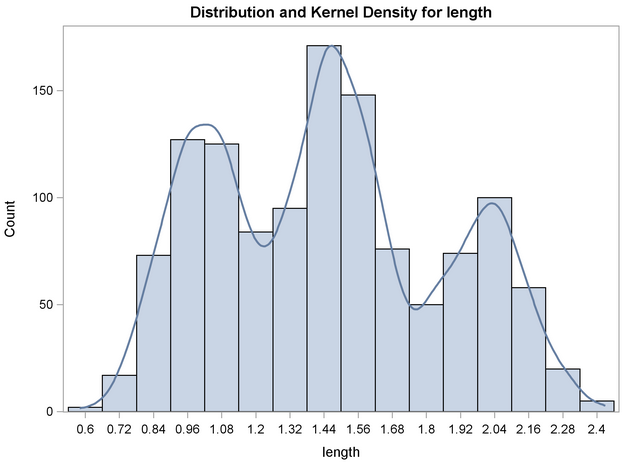
\includegraphics[scale=0.3]{images/Histogram.png}
\hspace{20 pt}
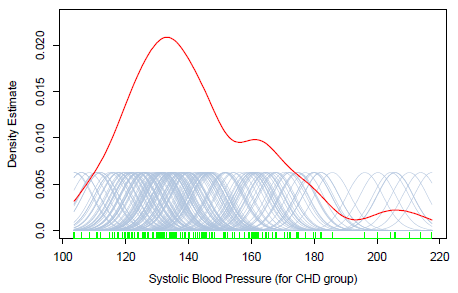
\includegraphics[scale=0.45]{images/GaussianKernel.png} \\
{\tiny \href{https://support.sas.com/documentation/cdl/en/statug/63033/HTML/default/viewer.htm}{https://support.sas.com/documentation/cdl/en/statug/63033/HTML/default/viewer.htm}} \\
{\tiny \href{https://web.stanford.edu/~hastie/Papers/ESLII.pdf}{https://web.stanford.edu/~hastie/Papers/ESLII.pdf}}
\end{frame}

\begin{frame}{KDE}
\centering
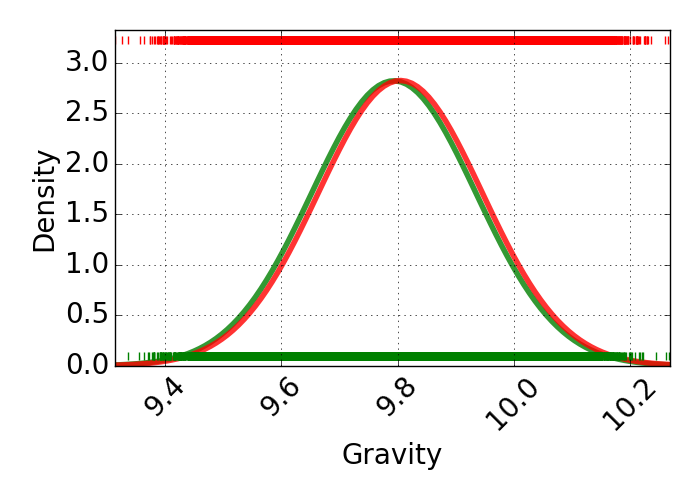
\includegraphics[scale=0.22]{images/KDE_Gravity.png}
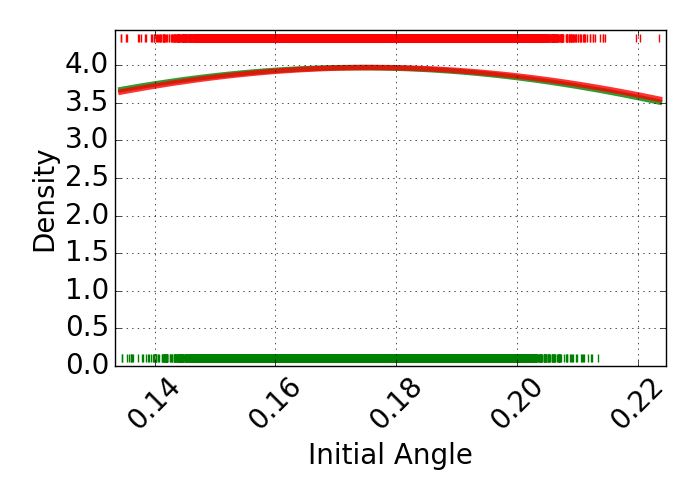
\includegraphics[scale=0.22]{images/KDE_InitialAngle.png}
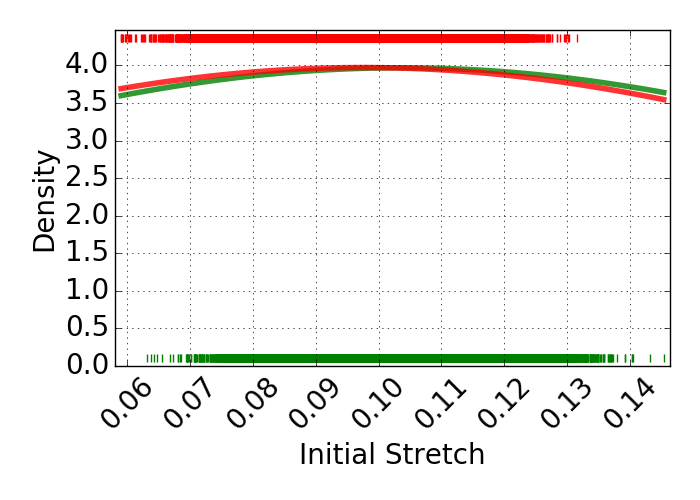
\includegraphics[scale=0.22]{images/KDE_InitialStretch.png}
\\
\vspace{10 pt}
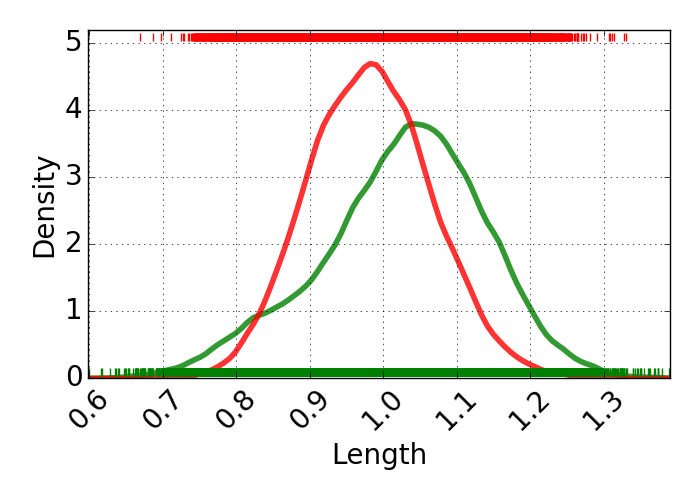
\includegraphics[scale=0.22]{images/KDE_Length.png}
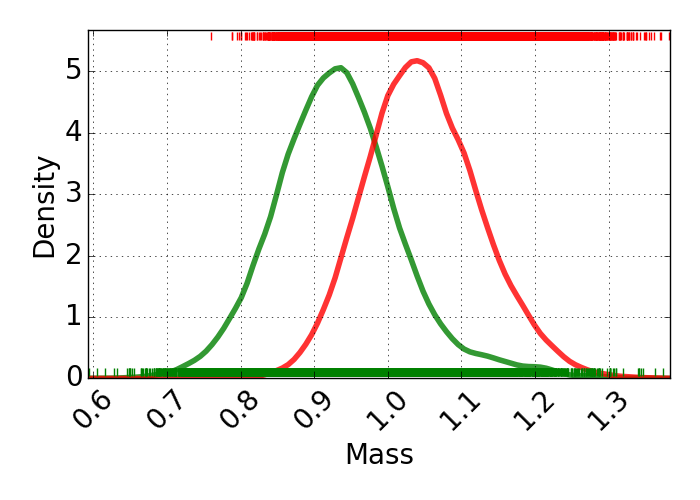
\includegraphics[scale=0.22]{images/KDE_Mass.png}
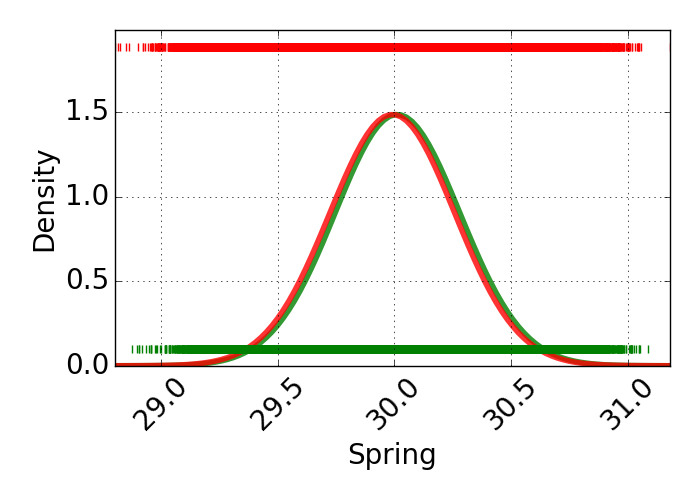
\includegraphics[scale=0.22]{images/KDE_Spring.png}
\end{frame}

\begin{frame}{K-Nearest Neighbors}
\centering
What is the k-nearest neighbor method? \\
\vspace{20 pt}
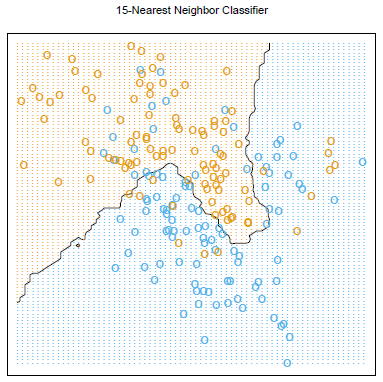
\includegraphics[scale=0.5]{images/KNNExample.png} \\
{\tiny \href{https://web.stanford.edu/~hastie/Papers/ESLII.pdf}{https://web.stanford.edu/~hastie/Papers/ESLII.pdf}}
\end{frame}

\begin{frame}{KNN}
\centering
\includegraphics[scale=0.27]{images/KNNPlot_Uniform.png}
\end{frame}

\begin{frame}{Accuracy}
\centering
\small
    \begin{tabular}{| c | c |}
    \hline
    Parameters & Accuracy \\ \hline
    Mass vs Length & 84.374\% \\ 
    Mass vs Initial Stretch & 79.264\% \\ 
    Mass vs Initial Angle & 74.108\% \\
    Mass vs Spring & 73.521\% \\    
    Mass vs Gravity & 73.196\% \\
    Length vs Initial Stretch & 65.593\% \\
    Length vs Spring & 59.245\% \\
    Length vs Gravity & 59.159\% \\
    Initial Stretch vs Spring & 59.155\% \\    
    Initial Angle vs Length & 59.144\% \\
    Initial Angle vs Initial Stretch & 59.129\% \\
    Initial Stretch vs Gravity & 57.850\% \\
    Initial Angle vs Gravity & 52.774\% \\
   Initial Angle vs Spring & 52.759\% \\
   Spring vs Gravity & 52.049\% \\ \hline
\end{tabular} 
%\includegraphics[scale=0.3]{images/KNN_UniAcc_HBars.png}
\end{frame}

\end{document}